\documentclass[11pt]{article}
\usepackage{amsmath} % AMS Math Package
\usepackage{polski}
\usepackage[utf8]{inputenc}
\usepackage{listings}
\usepackage{graphicx} % Allows for eps images
\newcommand{\png}[1]{\begin{center}\includegraphics{#1}\end{center}}
\newcommand{\largepng}[1]{\begin{center}\includegraphics[width=\linewidth]{#1}\end{center}}

\begin{document}
\largepng{tabelka.png}
\section{Zadanie 1}

Przy zestawie 3 oraz numerze indeksu 261604 proste obliczenia dają nam $\lambda=504 nm$. Światło monochromatyczne o tej długości
 fali ma kolor zielony.

Dla przejścia elektronu z pierwszego poziomu energetycznego w warstwie p do pierwszego poziomu energetycznego w warstwie n spełnione
 jest równanie:
\[E_{foton} = E_g + E_1n + E_1p\]

Gdzie $E_g$ jest przerwą energetyczną.

Poziomy energetyczne w warstwach można modelować poprzez nieskończoną studnię potencjału, znaną z mechaniki kwantowej, która,
 jak powszechnie wiadomo, ma energie:
\[E_n = \frac{\hbar^2}{2m} (\frac{n \pi}{d})^2 \]

Gdzie $d$ jest szerokością warstwy półprzewodnikowej w naszym jednowymiarowym przybliżeniu. Energia fotonu wyraża się zaś wzorem

\[E_{foton} = \frac{hc}{\lambda} \]

Przybliżając masy efektywne elektronów oraz dziur przez masę spoczynkową elektronu, otrzymujemy

\[ \frac{hc}{\lambda} = E_g + \frac{\hbar^2 \pi^2}{m_e d^2} \]

Przyjmując początkowo $d=5nm$, otrzymujemy przekształcając powyższy wzór $E_g=2.4299 eV$.

Za aktywny materiał półprzewodnikowy o zbliżonej do otrzymanej przerwy energetycznej wartości $E_g=2.42eV$
przyjmujemy siarczek kadmu $CdS$. Jego stałą sieciową odczytujemy z wykresu jako zawierającą się w przedziale $5.8-5.9 nm$.
Za materiał ``okładkowy'' przyjmujemy selenek magnezu $MgSe$ o stałej sieciowej z tego samego zakresu i energii przerwy około 4eV.
Schemat tej struktury wygladałby tak:

\begin{center}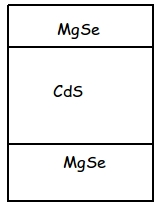
\includegraphics[width=90pt]{schemat.jpg}\end{center}
\section{Zadanie 2}

Dla danych z zestawu 3 współczynnik kształtu $l/S$ wynosi $1.04mm/1.89mm^2 = 0.05502/mm$.
Dane z pliku można przedstawić na wykresie Arrheniusa tak jak poniżej:
\largepng{z2.png}

Obliczenie współczynników przeprowadza się przy pomocy następującego skryptu w Pythonie:
\begin{lstlisting}[language=Python]
k = 1.38064852e-23
e = 1.60217662e-19
data = numpy.loadtxt("zad2_is_3_readable.txt")
Kelvin = 273.15
L=grubosc = 1.04e-3
S=powierzchnia = 18.9e-6
print(L/S)

T, R = temperatureC, resistanceOhm = data[:,0], data[:,1]
T+=Kelvin
G=1/R
conductivity = G*L/S

def linear_curve(x, a, b):
    return a*x+b
x = 1/T
y = np.log(conductivity*T/S)
coefficients, covs = scipy.optimize.curve_fit(linear_curve, x, y)
print(coefficients)
print(coefficients[0]*k/e)
\end{lstlisting}

Parametry dopasowania prostej $y=ax+b$ do zbioru danych $(1/T, \log{(\sigma T/S)}$ wynoszą:
\[a = 7153.0919 K, b = 26.6597\]

Co pozwala nam, mnożąc przez stałą Boltzmanna oraz dzieląc przez ładunek elektronu, otrzymać
\[ E_a = 0.6164 eV \]

Podstawiając otrzymane wartości ($\sigma_0 = \exp{b}$), otrzymujemy

\[ \sigma(25^{\circ}C) = 0.04834 S/m \]
% Wyznaczenie współczynnika kształtu próbki (tj. l/S)
% Wykreślenie danych w żądanych współrzędnych
% Oznaczenie wykresu (jednostki i opisy osi)
% Dopasowanie prostej i wyznaczenie parametrów dopasowania
% Obliczenie energii aktywacji
% Obliczenie wartości przewodności w 25 stopni C
\section{Zadanie 3}
Dla jednowymiarowej sieci krystalicznej którą modelujemy jako oscylatory harmoniczne
powiązane ze sobą sprężynami o stałej sieci $k$, w której to sieci komórka elementarna składa się
z dwóch połączonych ze sobą łańcuchowo atomów ("model bilardowy", tzn. klasyczny) o masach $m_1$ oraz $m_2$, można zapisać
odwołując się do drugiej zasady dynamiki\footnote{I. Newton, \textit{Principia...}}
układ równań ruchu dla obu atomów w $n$-tej komórce elementarnej, przyjmując $S_{in}$ jako odchylenie
$i (1, 2)$ atomu z $n$-tej komórki elementarnej z położenia równowagi:

\[m_1\ddot{S_{1n}} = k(S_{2n}+S_{2 (n-1)}) \]
\[m_2\ddot{S_{2n}} = k(S_{1n}+S_{1 (n+1)}) \]

Przymując, że odchylenia wyrażają się przez funkcje Blocha:
\[S = u(x)\exp{i(qna-\omega t)} \]
\[\ddot{S} = -\omega^2 S \]
Łatwo pokazać, że:
\[S_{n+1} = S \exp{(iqa)} \]
\[S_{n-1} S \exp{(-iqa)}\]
Przechodząc do pierwszej komórki elementarnej z racji jej okresowości:
\[ m_1 \omega^2 S_1 = k (S_2 + S_2 \exp{(-iqa)} \]
\[ m_2 \omega^2 S_2 = k (S_1 + S_1 \exp{(iqa)} \]
Wykonując proste przekształcenia, które pozostawiamy Czytelnikowi, otrzymujemy następujący układ równań:
\[ m_1 \omega^2 S_1 - k S_2 (1+\exp{(-iqa)}) = 0\]
\[ -k S_1 (1+\exp{(iqa)}) + m_2 \omega^2 S_2 = 0\]
Aby otrzymać dwa niezależne liniowo rozwiązania $S_1$ oraz $S_2$, wyznacznik tego wyrażenia musi się zerować:
\[(\frac{2k}{m_1}-\omega^2)(\frac{2k}{m_2}-\omega^2) - 2 \frac{k^2}{m_1 m_2} (1+\cos{(qa)}) = 0\]
Jest to oczywiście równanie dwukwadratowe, którego rozwiązaniami są dwie pary dodatnich i ujemnych $\omega$.
Rozwiązując to równanie\footnote{www.wolframalpha.com} i biorąc dodatnie $\omega$,
otrzymane funkcje można wykreślić dla pierwszej strefy Brillouina na poniższym wykresie:
\largepng{z3.png}
\end{document}
